
\documentclass[border=10pt, 12pt]{standalone}
\usepackage[svgnames]{xcolor}
\usepackage{amsmath}
\usepackage{pgfplots}
\pgfplotsset{compat=newest}
\usepackage[sfdefault]{FiraSans}
\usepackage{FiraMono}
\renewcommand*\familydefault{\sfdefault}
\begin{document}
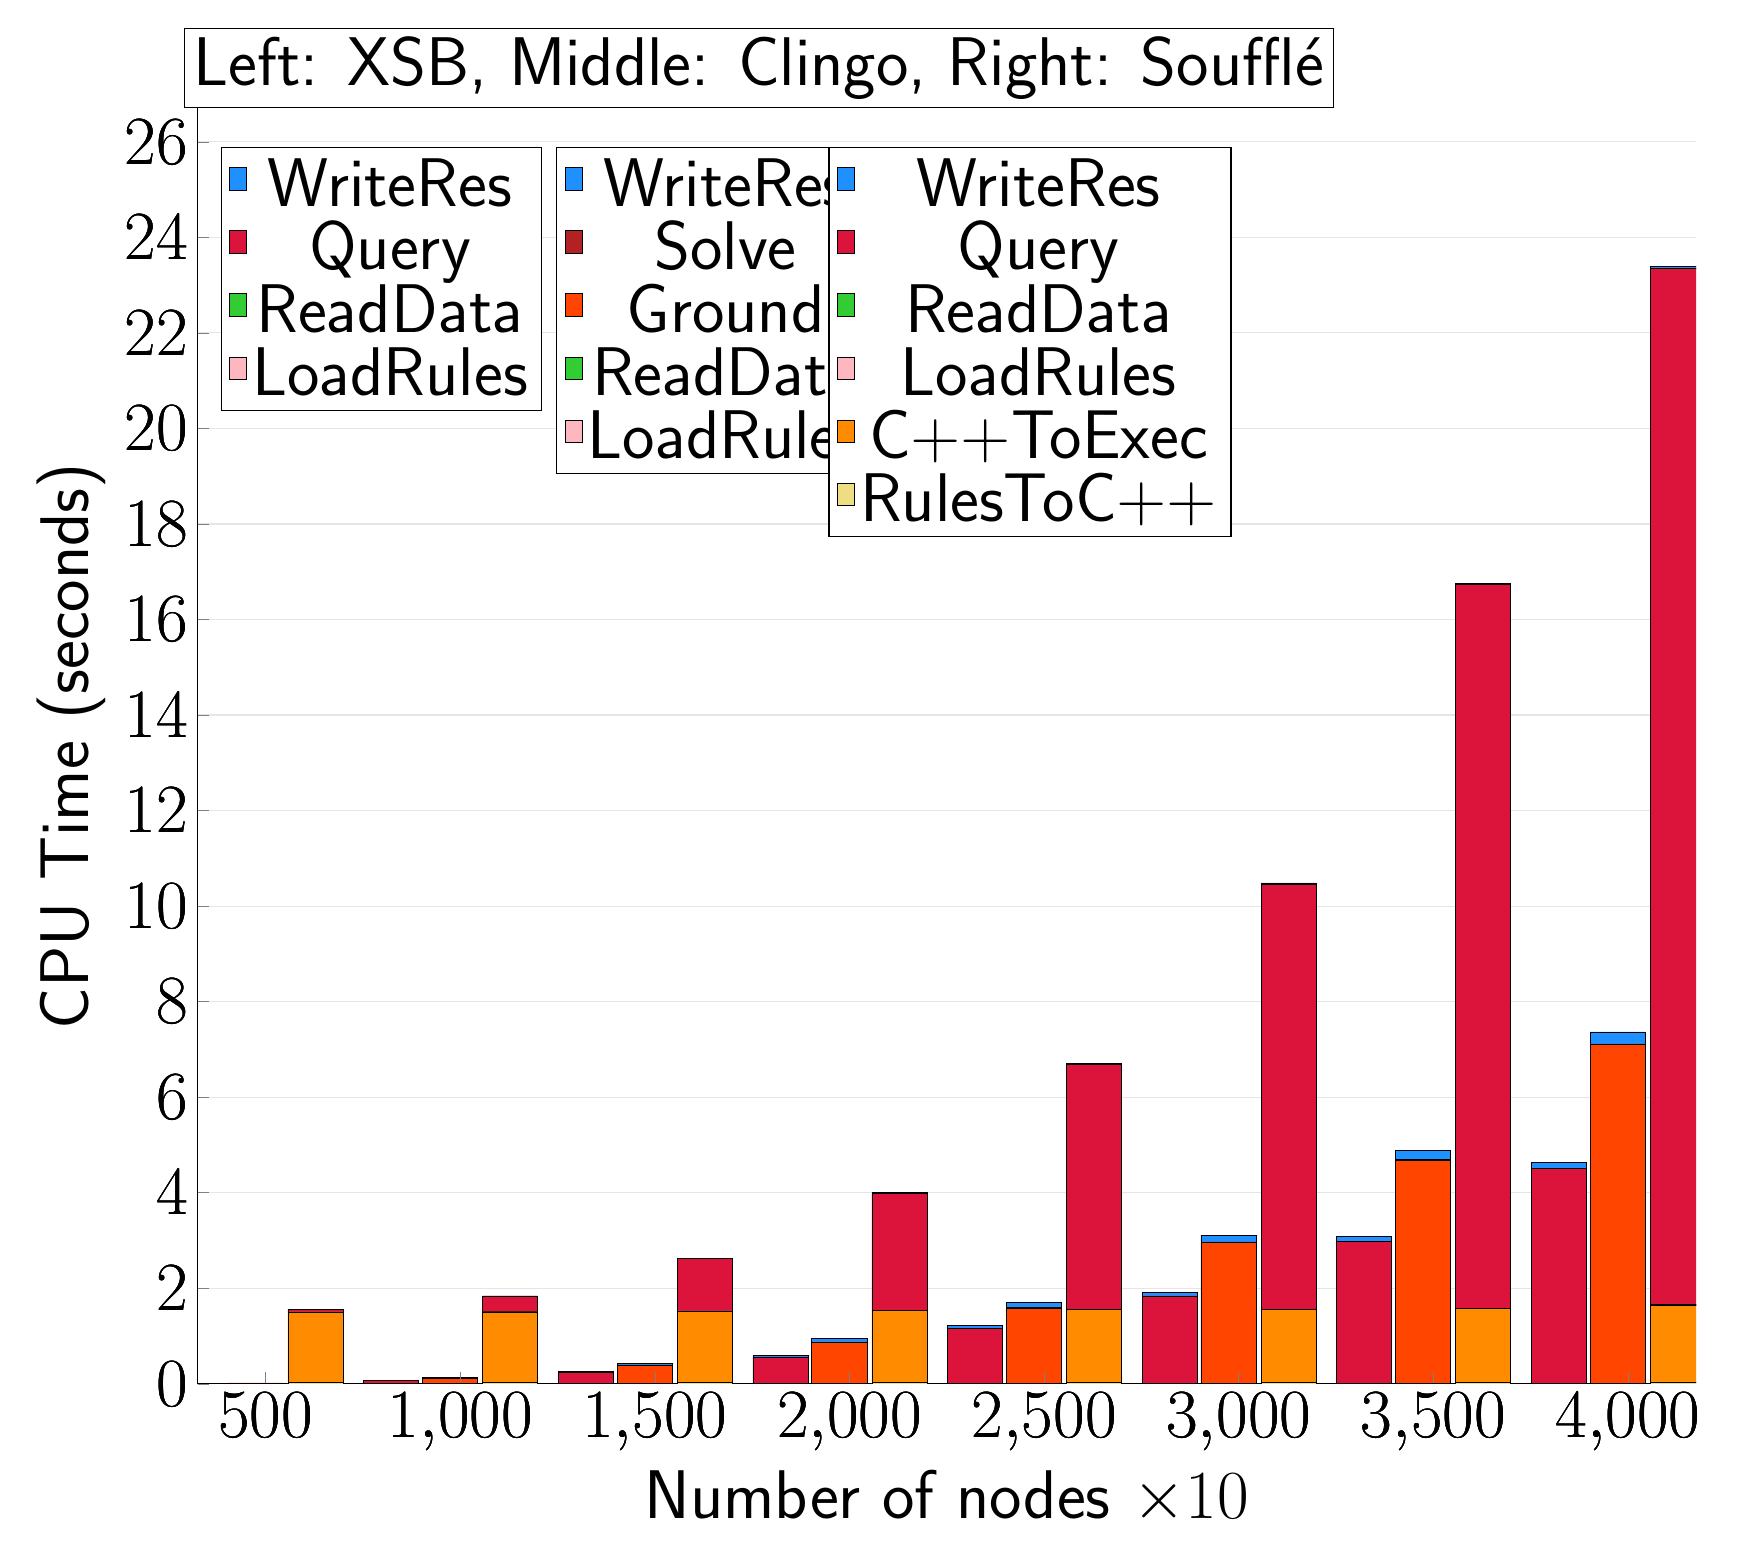
\begin{tikzpicture}
	\begin{axis}[bar shift=-25pt,
			ybar stacked,
			width=1.7\textwidth,
			bar width=0.7cm,
			ymajorgrids, tick align=inside,
			major grid style={draw=gray!20},
			xtick=data,
			ymin=0, ymax=26.698890000000002,
			axis x line*=bottom,
			axis y line*=left,
			enlarge x limits=0.05,
			legend style={
					at={(0.23, 0.97)},
					anchor=north east,
					legend columns=1,
					font=\Huge,
				},
			ylabel={CPU Time (seconds)},
			xlabel={Number of nodes $\times 10$},
			label style={font=\Huge},
			tick label style={font=\Huge},
		]
		\addlegendimage{fill=DodgerBlue, draw=black, line width=0.2pt}
		\addlegendentry{WriteRes}
		\addlegendimage{fill=Crimson, draw=black, line width=0.2pt}
		\addlegendentry{Query}
		\addlegendimage{fill=LimeGreen, draw=black, line width=0.2pt}
		\addlegendentry{ReadData}
		\addlegendimage{fill=LightPink, draw=black, line width=0.2pt}
		\addlegendentry{LoadRules}
		\addplot +[fill=LightPink, draw=black, line width=0.2pt] coordinates {
				(500, 0.0006204)
				(1000, 0.0006066000000000002)
				(1500, 0.0006002000000000001)
				(2000, 0.0006371000000000004)
				(2500, 0.0006150999999999997)
				(3000, 0.0006217)
				(3500, 0.0006406000000000001)
				(4000, 0.0006160000000000001)
			};
		\addplot +[fill=LimeGreen, draw=black, line width=0.2pt] coordinates {
				(500, 0.0005870999999999995)
				(1000, 0.0010638)
				(1500, 0.0015355)
				(2000, 0.0020614)
				(2500, 0.0026220999999999996)
				(3000, 0.0030441)
				(3500, 0.0035825999999999996)
				(4000, 0.0039934)
			};
		\addplot +[fill=Crimson, draw=black, line width=0.2pt] coordinates {
				(500, 0.007741)
				(1000, 0.06547050000000001)
				(1500, 0.23226030000000003)
				(2000, 0.5598783999999999)
				(2500, 1.1648720000000001)
				(3000, 1.8355333000000003)
				(3500, 2.9813151)
				(4000, 4.500052500000001)
			};
		\addplot +[fill=DodgerBlue, draw=black, line width=0.2pt] coordinates {
				(500, 0.0022398000000000006)
				(1000, 0.009411700000000002)
				(1500, 0.022235599999999994)
				(2000, 0.034432000000000004)
				(2500, 0.05318070000000001)
				(3000, 0.0781804)
				(3500, 0.10023200000000002)
				(4000, 0.13836970000000015)
			};
	\end{axis}

	\begin{axis}[bar shift=-3.7pt,
			ybar stacked,
			width=1.7\textwidth,
			bar width=0.7cm,
			ymajorgrids, tick align=inside,
			major grid style={draw=none},
			xtick=data,
			ymin=0, ymax=26.698890000000002,
			axis x line*=none,
			axis y line*=none,
			enlarge x limits=0.05,
			legend style={
					at={(0.454, 0.97)},
					anchor=north east,
					legend columns=1,
					font=\Huge,
				},
			label style={font=\Huge},
			tick label style={font=\Huge},
		]
		\addlegendimage{fill=DodgerBlue, draw=black, line width=0.2pt}
		\addlegendentry{WriteRes}
		\addlegendimage{fill=FireBrick, draw=black, line width=0.2pt}
		\addlegendentry{Solve}
		\addlegendimage{fill=OrangeRed, draw=black, line width=0.2pt}
		\addlegendentry{Ground}
		\addlegendimage{fill=LimeGreen, draw=black, line width=0.2pt}
		\addlegendentry{ReadData}
		\addlegendimage{fill=LightPink, draw=black, line width=0.2pt}
		\addlegendentry{LoadRules}
		\addplot +[fill=LightPink, draw=black, line width=0.2pt] coordinates {
				(500, 0.0)
				(1000, 0.0)
				(1500, 0.0)
				(2000, 0.0)
				(2500, 0.0)
				(3000, 0.0)
				(3500, 0.0)
				(4000, 0.0)
			};
		\addplot +[fill=LimeGreen, draw=black, line width=0.2pt] coordinates {
				(500, 0.0)
				(1000, 0.0)
				(1500, 0.009999999999999997)
				(2000, 0.008999999999999998)
				(2500, 0.009999999999999997)
				(3000, 0.009999999999999997)
				(3500, 0.010999999999999998)
				(4000, 0.009999999999999997)
			};
		\addplot +[fill=OrangeRed, draw=black, line width=0.2pt] coordinates {
				(500, 0.019999999999999997)
				(1000, 0.11800000000000002)
				(1500, 0.383)
				(2000, 0.8709999999999999)
				(2500, 1.5800000000000003)
				(3000, 2.9519999999999995)
				(3500, 4.667999999999999)
				(4000, 7.0920000000000005)
			};
		\addplot +[fill=FireBrick, draw=black, line width=0.2pt] coordinates {
				(500, 0.0)
				(1000, 0.0020000000000000018)
				(1500, 0.002999999999999997)
				(2000, 0.0)
				(2500, 0.0020000000000000018)
				(3000, 0.009999999999999943)
				(3500, 0.013000000000000123)
				(4000, 0.016000000000000014)
			};
		\addplot +[fill=DodgerBlue, draw=black, line width=0.2pt] coordinates {
				(500, 0.0)
				(1000, 0.010999999999999992)
				(1500, 0.032000000000000015)
				(2000, 0.07199999999999998)
				(2500, 0.10799999999999992)
				(3000, 0.14200000000000007)
				(3500, 0.19499999999999976)
				(4000, 0.24900000000000003)
			};
	\end{axis}

	\begin{axis}[bar shift=18pt,
			ybar stacked,
			width=1.7\textwidth,
			bar width=0.7cm,
			ymajorgrids, tick align=inside,
			major grid style={draw=none},
			xtick=data,
			ymin=0, ymax=26.698890000000002,
			axis x line*=none,
			axis y line*=none,
			enlarge x limits=0.05,
			legend style={
					at={(0.69, 0.97)},
					anchor=north east,
					legend columns=1,
					font=\Huge,
				},
			label style={font=\Huge},
			tick label style={font=\Huge},
		]
		\addlegendimage{fill=DodgerBlue, draw=black, line width=0.2pt}
		\addlegendentry{WriteRes}
		\addlegendimage{fill=Crimson, draw=black, line width=0.2pt}
		\addlegendentry{Query}
		\addlegendimage{fill=LimeGreen, draw=black, line width=0.2pt}
		\addlegendentry{ReadData}
		\addlegendimage{fill=LightPink, draw=black, line width=0.2pt}
		\addlegendentry{LoadRules}
		\addlegendimage{fill=DarkOrange, draw=black, line width=0.2pt}
		\addlegendentry{C++ToExec}
		\addlegendimage{fill=LightGoldenrod, draw=black, line width=0.2pt}
		\addlegendentry{RulesToC++}
		\addplot +[fill=LightGoldenrod, draw=black, line width=0.2pt] coordinates {
				(500, 0.030000000000000006)
				(1000, 0.030000000000000006)
				(1500, 0.030000000000000006)
				(2000, 0.030000000000000006)
				(2500, 0.031000000000000007)
				(3000, 0.031000000000000007)
				(3500, 0.036)
				(4000, 0.041999999999999996)
			};
		\addplot +[fill=DarkOrange, draw=black, line width=0.2pt] coordinates {
				(500, 1.473)
				(1000, 1.4760000000000002)
				(1500, 1.4920000000000002)
				(2000, 1.504)
				(2500, 1.5240000000000002)
				(3000, 1.525)
				(3500, 1.539)
				(4000, 1.605)
			};
		\addplot +[fill=LightPink, draw=black, line width=0.2pt] coordinates {
				(500, 9.609999999999999e-05)
				(1000, 8.65e-05)
				(1500, 6.63e-05)
				(2000, 3.33e-05)
				(2500, 5.22e-05)
				(3000, 0.0001088)
				(3500, 9.77e-05)
				(4000, 6.45e-05)
			};
		\addplot +[fill=LimeGreen, draw=black, line width=0.2pt] coordinates {
				(500, 0.0014632)
				(1000, 0.0026191)
				(1500, 0.0035453)
				(2000, 0.0044359)
				(2500, 0.005587399999999999)
				(3000, 0.0064504)
				(3500, 0.0079138)
				(4000, 0.008193200000000001)
			};
		\addplot +[fill=Crimson, draw=black, line width=0.2pt] coordinates {
				(500, 0.0535867)
				(1000, 0.3307171)
				(1500, 1.095862)
				(2000, 2.450427)
				(2500, 5.131427)
				(3000, 8.899659)
				(3500, 15.14585)
				(4000, 21.698890000000002)
			};
		\addplot +[fill=DodgerBlue, draw=black, line width=0.2pt] coordinates {
				(500, 0.0009061)
				(1000, 0.0029717)
				(1500, 0.0065487)
				(2000, 0.011430899999999999)
				(2500, 0.017599999999999998)
				(3000, 0.025351999999999996)
				(3500, 0.034351900000000005)
				(4000, 0.04497399999999999)
			};
	\end{axis}


	\node[anchor=south, draw, fill=white] at (rel axis cs:0.42,1) {\Huge Left: XSB, Middle: Clingo, Right: Soufflé};
\end{tikzpicture}
\end{document}
